\documentclass[12pt]{article}

\usepackage[margin=1in]{geometry}
\usepackage[version=3]{mhchem}
\usepackage{graphicx}
\usepackage{subfig}
\usepackage{fancyhdr}
\usepackage{amsmath}



\newcommand{\unit}[1]{\ensuremath{\, \mathrm{#1}}}
\newcommand{\e}[1]{\ensuremath{\times 10^{#1}}}

\pagestyle{fancy}
\lhead{NANO 266 - Quantum Mechanical Modeling}
\rhead{Spring 2015}

\title{NANO 266 - Lab 4}
\author{Zhi Deng \\ PID:A53058446}
\date{June 5, 2015}

\begin{document}

\maketitle
\thispagestyle{fancy}

\section*{Q1}

\subsection*{1}

Find the lattice constant of fcc Al at equilibrium using the SCF method. 

\begin{figure}[h]
\begin{center}
	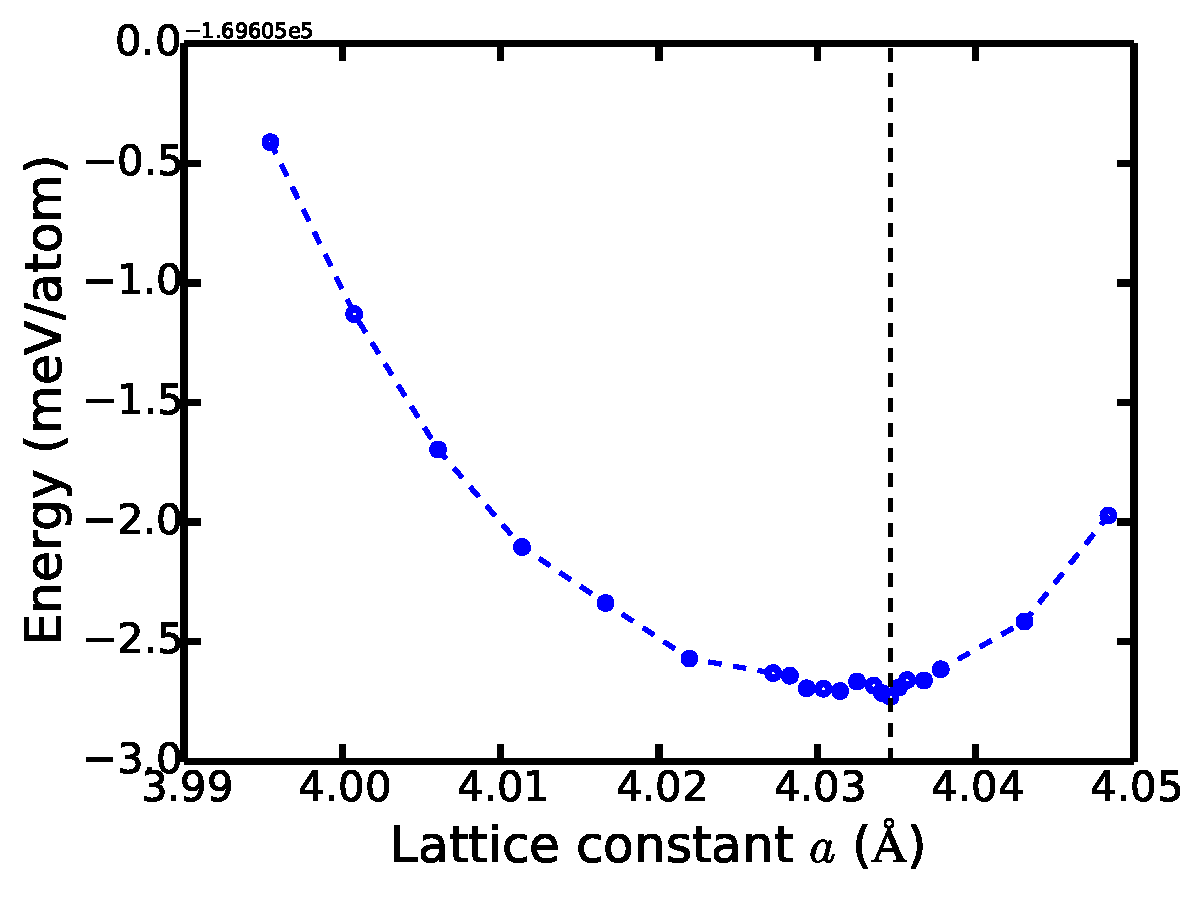
\includegraphics[width=.6\textwidth]{Al_latt}
\end{center}
\end{figure}

The lattice constant $a_0 = 7.624\unit{a.u.} = 4.0346\unit{\AA}$. The horrible shape is probably due to the choice of  low energy cut-off. Record the total energy at equilibrium lattice constant for surface energy calculations. 

\subsection*{2}

Find the numbers of vacuum layers and slab layers needed for a converged surface energy of Al $(100)$. The surface energy is calculated from the following equation: 
\begin{flalign*}
	\gamma = \frac{1}{2A}(E_{\rm slab} - NE_{\rm bulk})
\end{flalign*}
where $A$ is the cross-section area of that tetragonal simulation box ($A = a_0^2$), $E_{\rm slab}$ is the total energy of the entire slab, $N$ is the number of atoms in the slab and $E_{\rm bulk}$ is the energy of bulk Al per atom (calculated in 1). 

With the number of slab layers fixed to 2, vary the number of vacuum layers. The result shows that the surface energy converges within $0.01\unit{J/m^2}$ when the number of vacuum layers reaches 3. 

\begin{figure}[h]
\begin{center}
	\subfloat{
		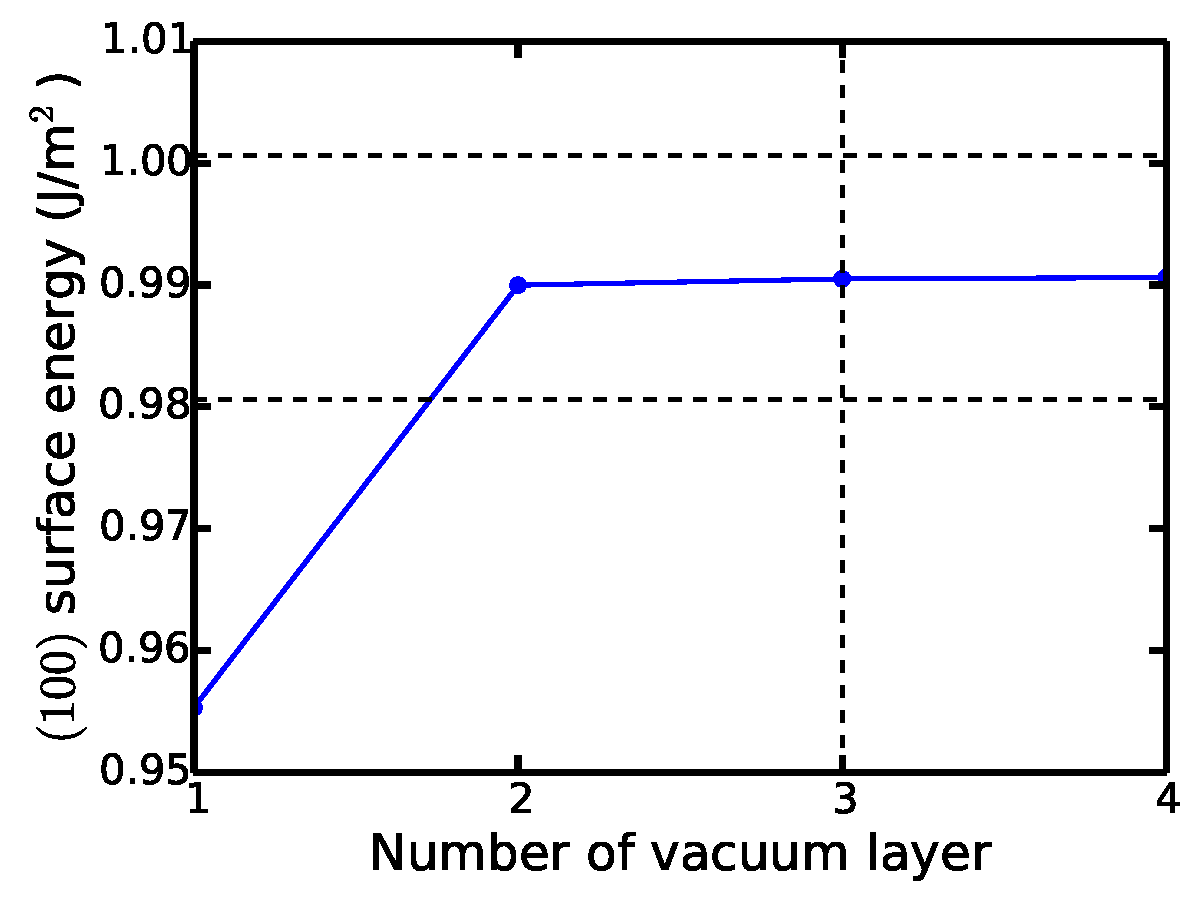
\includegraphics[width=.45\textwidth]{Al_100_nvac}
	}
	\quad
	\subfloat{
		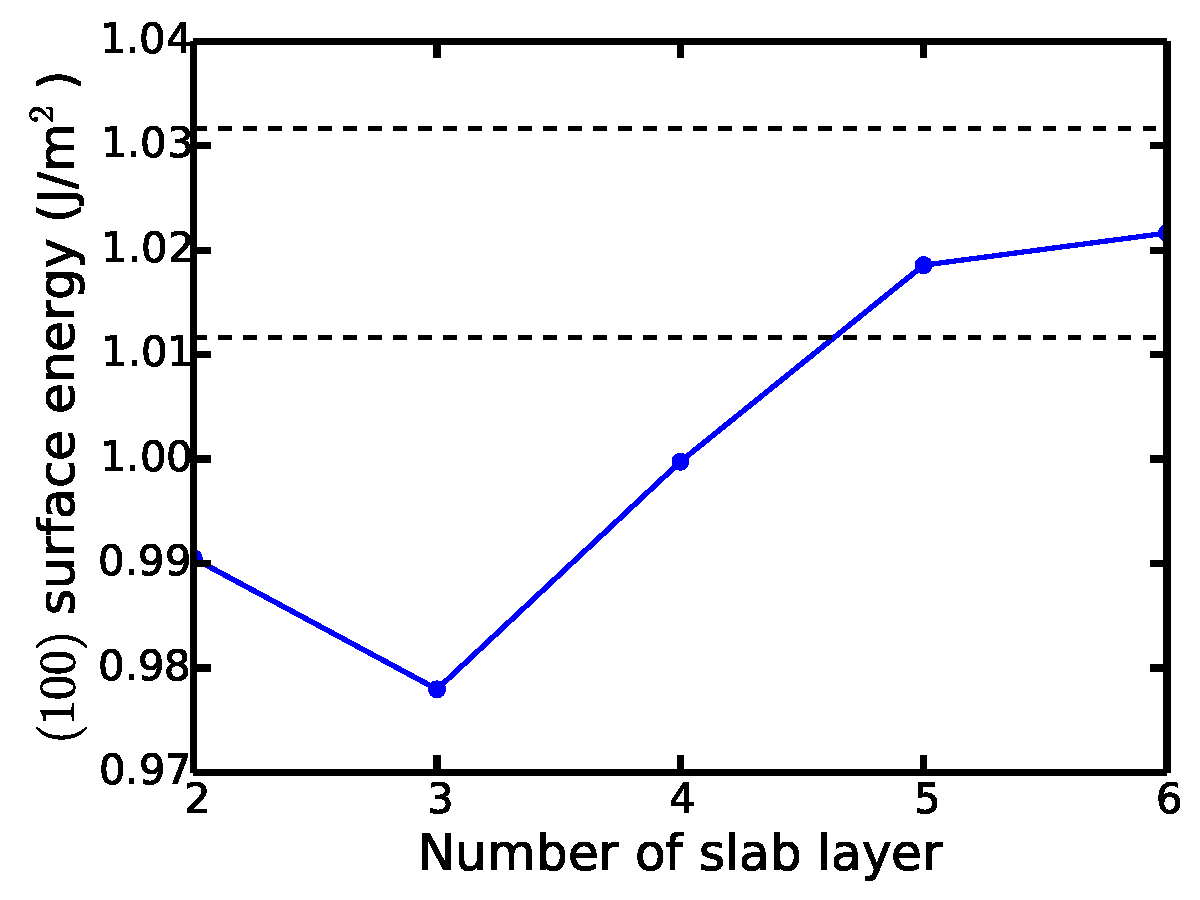
\includegraphics[width=.45\textwidth]{Al_100_nslab}
	}
\end{center}
\end{figure}

With the number of vacuum layers set to 3, vary the number of slab layers. The result shows that the surface energy
the surface energy converges within $0.01\unit{J/m^2}$ when the number of slab layers reaches 6. 

Therefore, the surface energy of Al $(100)$ $\gamma_{100} = 1.022\unit{J/m^2}$. 

Visualize the final relaxed slab in VESTA. Except for minor displacements in the $c$ direction, no obvious surface reconstruction is observed, probably due to the small cell size in $a$ and $b$ direction. 

\begin{figure}[h]
\begin{center}
	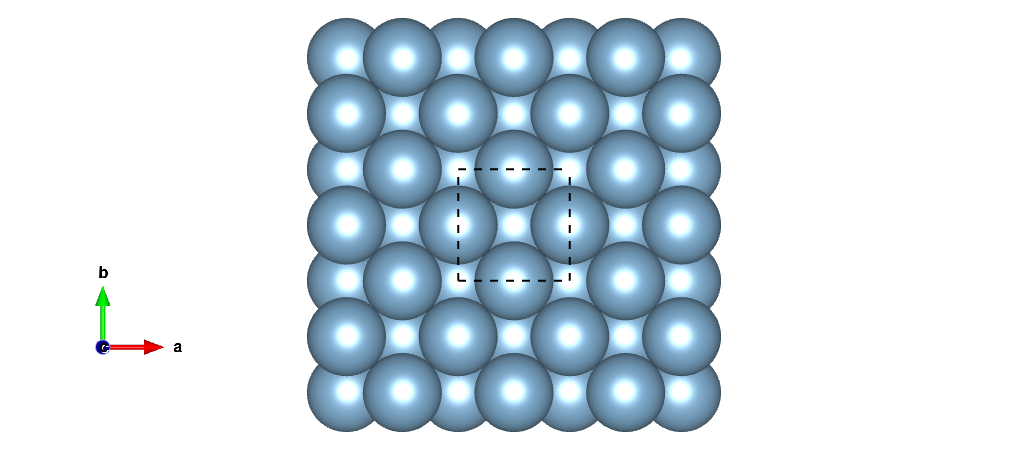
\includegraphics[width=.8\textwidth]{100.png}
\end{center}
\end{figure}

\section*{Q2}

Calculate the surface energy of Al $(111)$ with a hexagonal lattice setting, in which the lattice parameter $a = a_0/\sqrt{2} = 5.391\unit{a.u.} = 2.8529\unit{\AA}$ and the cross-section area $A = \sqrt{3}a^2/2$. 

Using a cell with 3 layers of slab and 2 layers of vacuum, the surface energy for Al $(111)$ $\gamma_{111} = 0.864\unit{J/m^2}$. 

Visualize the final relaxed slab in VESTA. Similarly, except for minor displacements in the $c$ direction, no obvious surface reconstruction is observed, probably due to the small cell size in $a$ and $b$ direction. 

\begin{figure}[h]
\begin{center}
	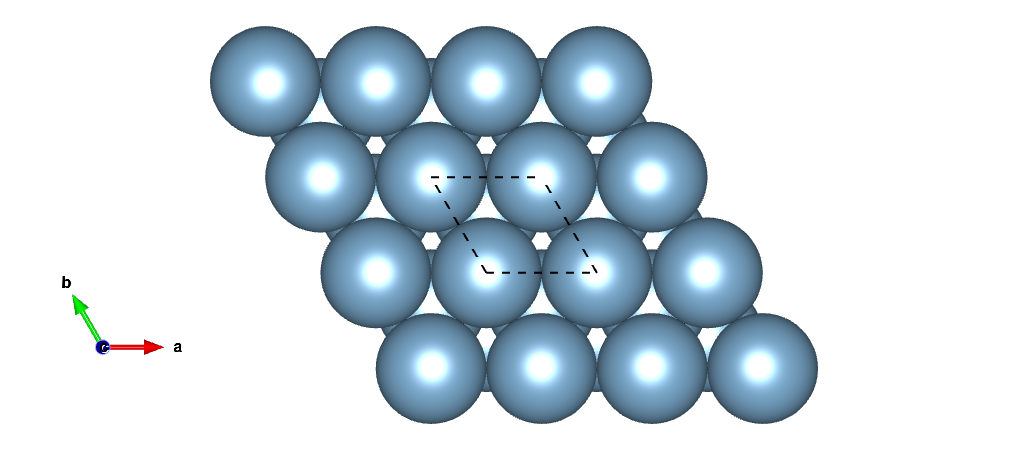
\includegraphics[width=.8\textwidth]{111.png}
\end{center}
\end{figure}

Al $(111)$ has lower surface energy than Al $(100)$. The reason is that $(111)$ is more closely packed. As a result, during the surface creation, less energy is needed with fewer nearest neighbor bonds cleaved within unit area. 

\section*{Q3}

The binding energy of H on Al $(111)$ surface is given by:
\begin{flalign*}
	E_{\rm b} = E_{\rm slab+H} - E_{\rm slab} - \frac{1}{2}E_\ce{H2}
\end{flalign*}
where $E_{\rm slab+H}$ is the energy of slab with H atom absorbed, $E_{\rm slab}$ is the energy of pure slab (calculated in Q2), $E_\ce{H2}$ is the energy of a single \ce{H2} molecule. 

Calculate $E_\ce{H2}$ using a simple cubic simulation box around 10\unit{\AA} and a minimal $1\times1\times1$ $k$-point grid. Convergence test with minor variations in box size shows that the cell size chosen is sufficient to converge the energy within 1\unit{meV}. 

There are 4 types of absorption sites on the Al $(111)$ shown in the figure below. The difference between the 2 hollow sites is that there is no Al atom at the same position in the layer underneath the surface layer for hollow1. Calculate $E_{\rm slab+H}$ with various absorption sites using a $2\times2\times1$ supercell generated from the relaxed slab in Q2. Since the lattice parameters $a$ and $b$ are doubled, an $8\times8\times1$ $k$-point grid is chosen. 
\clearpage

\begin{figure}[h]
\begin{center}
	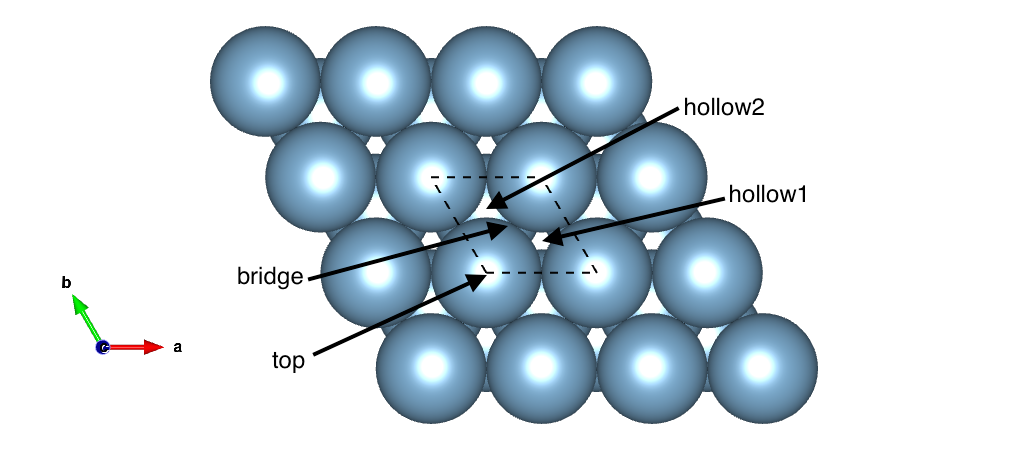
\includegraphics[width=.8\textwidth]{sites.png}
\end{center}
\end{figure}

Visualize the slab with H atom absorbed after relaxation. Multiple H atoms are periodic images due to the limited cell size. Most final geometries are really close to their corresponding initial guesses except for the H atom on bridge site. It falls into the nearest hollow1 site eventually.  

\begin{figure}[h]
\begin{center}
	\subfloat[top]{
		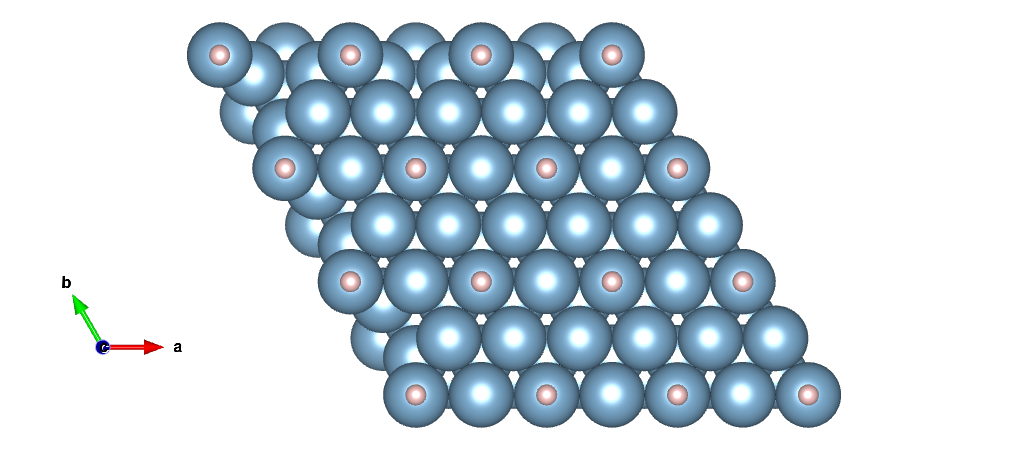
\includegraphics[trim=6.5cm 0 6.5cm 0,clip,width=.35\textwidth]{top_r.png}
	}
	\subfloat[bridge]{
		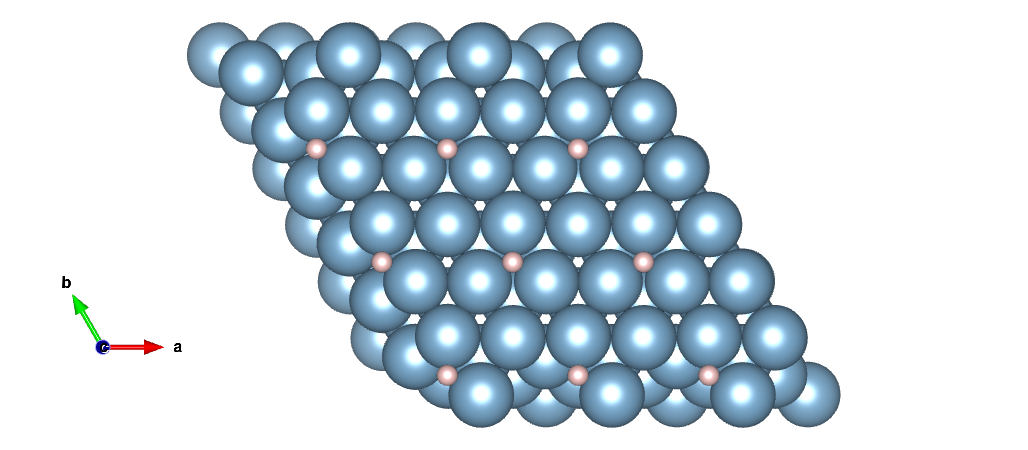
\includegraphics[trim=6.5cm 0 6.5cm 0,clip,width=.35\textwidth]{bridge_r.png}
	}
	\quad
	\subfloat[hollow1]{
		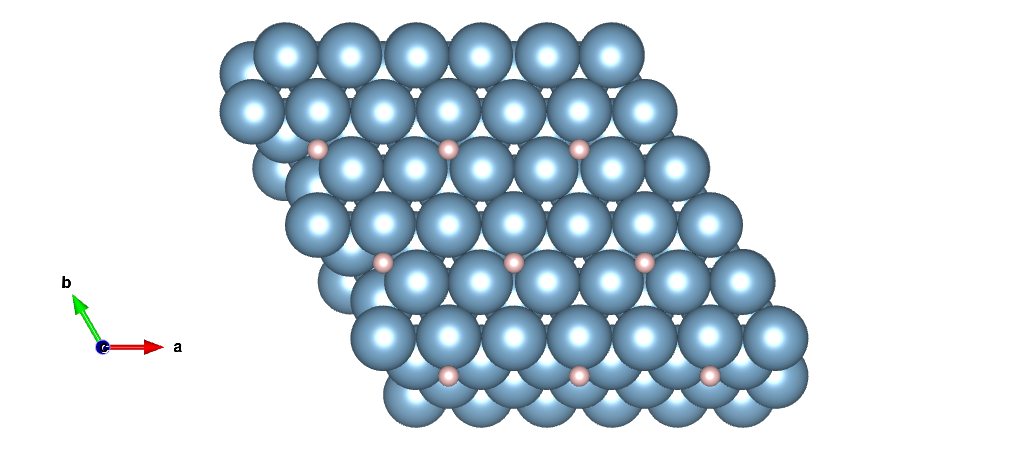
\includegraphics[trim=6.5cm 0 6.5cm 0,clip,width=.35\textwidth]{hollow1_r.png}
	}
	\subfloat[hollow2]{
		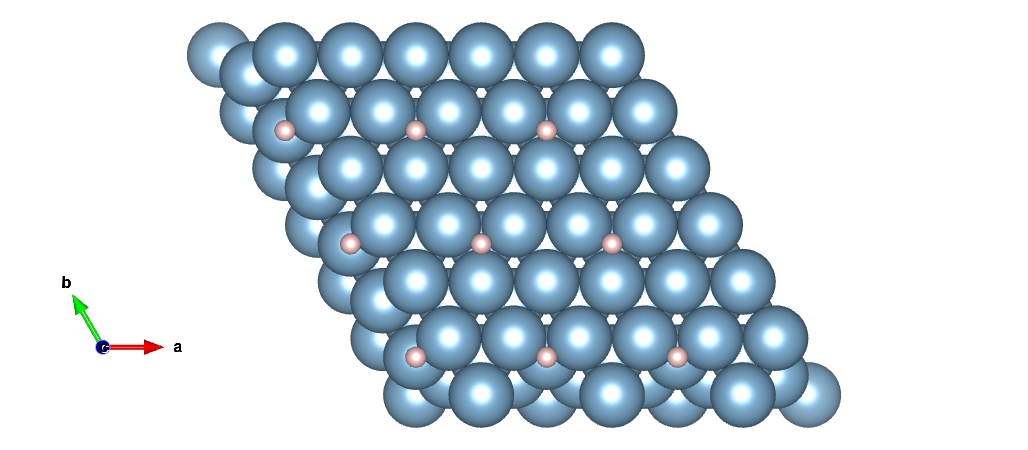
\includegraphics[trim=6.5cm 0 6.5cm 0,clip,width=.35\textwidth]{hollow2_r.png}
	}
\end{center}
\end{figure}

To get $E_{\rm slab+H}$ on the bridge site, constrain the force on H in $a$-$b$ plane. The final geometry is shown below. 
\clearpage

\begin{figure}[h]
\begin{center}
	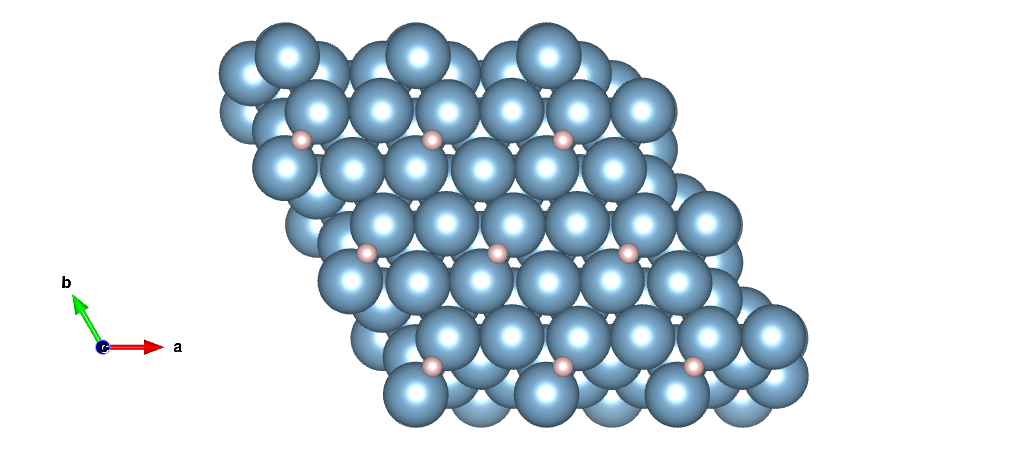
\includegraphics[trim=6.5cm 0 6.5cm 0,clip,width=.4\textwidth]{bridge_c.png}
\end{center}
\end{figure}

Now the H atom is sitting well on the bridge site. 

Calculate the binding energy of H from various absorption sites. 

\begin{figure}[h]
\begin{center}
	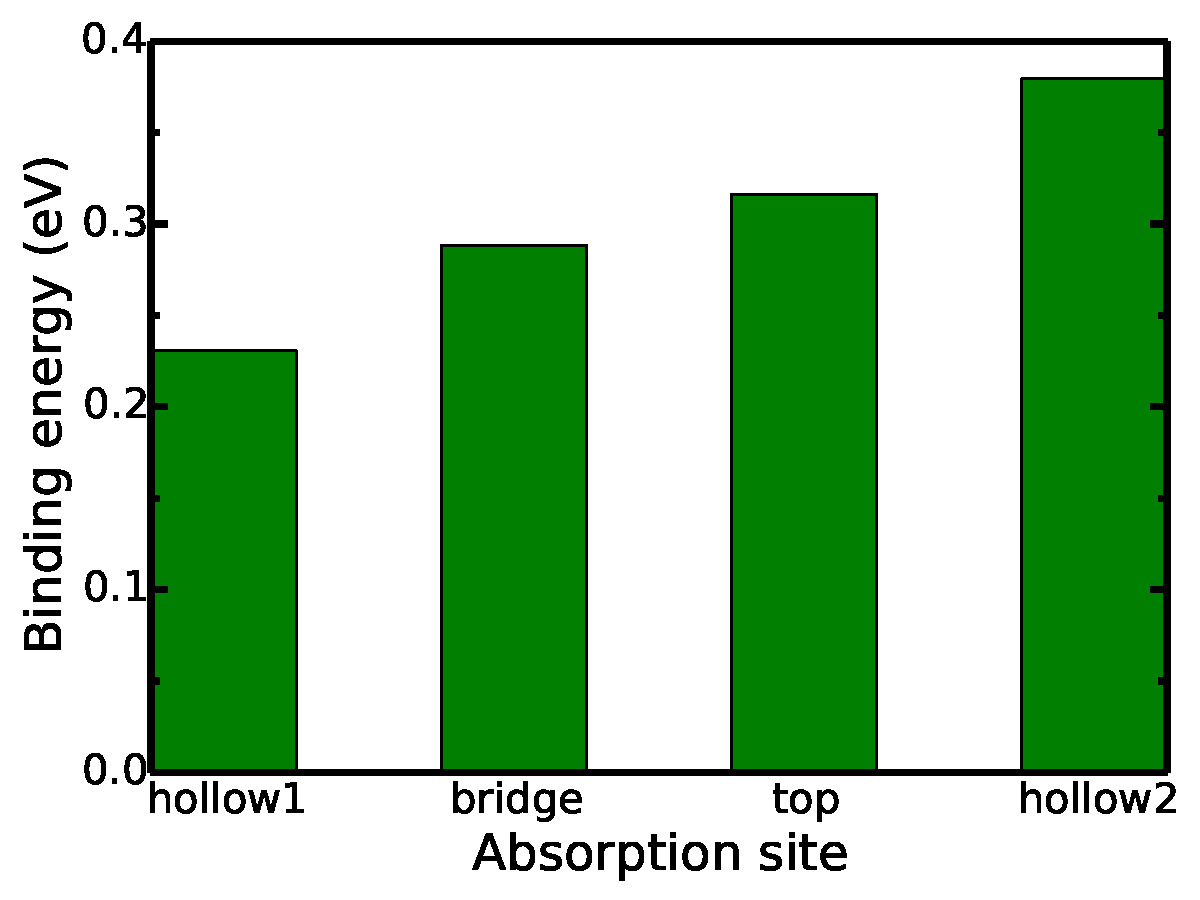
\includegraphics[width=.6\textwidth]{e_bind}
\end{center}
\end{figure}

Hollow2 site has the highest binding energy coming from the strong repulsion of the Al atom right underneath it as well as that from 3 Al atoms surrounding it in the surface. While for the top site without any surrounding Al atoms, the binding energy is still high due the Al atom right underneath it. The hollow1 site does not have any Al atom right underneath it, thus having the lowest binding energy. And the absorption on bridge site is highly unstable due to the energy gradient between the 2 hollow site. 

We can construct two types of migration pathways connecting 2 hollow1 sites: 
\begin{itemize}
	\item Path1: hollow1 - top - hollow1
	\item Path2: hollow1 - hollow2 - hollow1
\end{itemize}
Apparently, the barrier of path1 is lower than that of path2, making path1 more likely to be the dominant migration path for H on Al $(111)$ surface. 

The diffusion coefficient of H on Al $(111)$ can be roughly estimated using the following equation: 
\begin{flalign*}
	D = \frac{\nu r^2}{z}
\end{flalign*}
where $\nu$ is the hopping frequency, $r$ is jumping distance between 2 neighbor hollow1 sites ($r = a_0/\sqrt{2}$) and $z$ is the number of nearest neighbors ($z = 6$ for hexagonal Al $(111)$). $\nu$ can be calculated using the following equation: 
\begin{flalign*}
	\nu = \nu_0\exp\left(-\frac{\Delta E}{kT}\right)
\end{flalign*}
where $\nu_0$ is the oscillation frequency of H atom ($\nu_0 \sim 10^{13}\unit{s^{-1}}$), $\Delta E$ is the migration barrier (binding energy difference between hollow1 and top site), $k$ is the Boltzmann constant and $T$ is the temperature. 

\end{document}